% This file is part of sydetex.

% sydetex is free software: you can redistribute it and/or modify
% it under the terms of the GNU General Public License as published by
% the Free Software Foundation, either version 3 of the License, or
% any later version.

% sydetex is distributed in the hope that it will be useful,
% but WITHOUT ANY WARRANTY; without even the implied warranty of
% MERCHANTABILITY or FITNESS FOR A PARTICULAR PURPOSE.  See the
% GNU General Public License for more details.

% You should have received a copy of the GNU General Public License
% along with sydetex.  If not, see <https://www.gnu.org/licenses/>.


\documentclass[12pt]{article}
\usepackage[utf8]{inputenc}
\usepackage{setspace}



% THIS IS WHERE ALL THE SYDE STUFF IS
\usepackage{sydestyle}



% Reference tooling package settings - point to where the files are
\graphicspath{{figures/}}

\addbibresource{references.bib}

\makeglossaries
\newglossaryentry{tits} 
{
    name=tits,
    description={The tits, chickadees, and titmice constitute the Paridae, a large family of small passerine birds which occur mainly in the Northern Hemisphere and Africa. Most were formerly classified in the genus Parus. While commonly referred to as "tits" throughout much of the English-speaking world, these birds are called either "chickadees" (onomatopoeic, derived from their distinctive "chick-a dee dee dee" alarm call)[1] or "titmice" in North America. The name titmouse is recorded from the 14th century, composed of the Old English name for the bird, mase (Proto-Germanic *maison, German Meise), and tit, denoting something small. The former spelling, "titmose", was influenced by mouse in the 16th century.[2] Emigrants to New Zealand presumably identified some of the superficially similar birds of the genus Petroica of the family Petroicidae, the Australian robins, as members of the tit family, giving them the title tomtit, although, in fact, they are not related. }
}

\newglossaryentry{math}
{
    name=mathematics,
    description={Mathematics is what mathematicians do}
}

\newglossaryentry{formula}
{
    name=formula,
    description={A mathematical expression}
}

\newacronym{gcd}{GCD}{Greatest Common Divisor}

\newacronym{lcm}{LCM}{Least Common Multiple}

\newacronym{api}{API}{Application Programming Interface}


% hyperref is a prissy princess, so we import it here to prevent weirdness with sydetex.sty
\usepackage{hyperref}
\hypersetup{
    bookmarks=false
}



% PERSONAL DETAILS HERE, this sets up title page
\def\reportTitle{Fancy Title for Some Trivial Thing You Did}
\def\reportDueDate{April 1, 1969}
\def\studentName{Your Name}
\def\studentNumber{69696969}
\def\company{Your Company}
\def\lastSemester{3A}



% Form fitting ;)
\title{\reportTitle}
\author{\studentName}
\studentnumber{\studentNumber}
\lastsemester{\lastSemester}
\date{\reportDueDate}
\employer{\company}
\employeraddress{123 Muffin Lane \\ Hupperdook, ON A1A 1A1}



% ------------------------------START OF DOCUMENT------------------------------

% You shouldn't need to edit code above this line for the template to work as 
% intended. Just fill in your content and it should work Just Like Magic (TM).

\begin{document}

    
    \startindent
	\makewtrtitle
	\stopindent
	
	
	\begin{singlespace}

		YOUR RETURN ADDRESS HERE \\

    	April 1, 1969

		% TODO: CHECK ME IF IT'S STILL FIEGUTH
		Dr. Paul Fieguth, Professor and Department Chair
	
		Systems Design Engineering
	
	    University of Waterloo
	
	    Waterloo, ON
	
	    N2L 3G1\\
	
		Dear Professor Fieguth,
	\end{singlespace}
    
        I have prepared this report, “\reportTitle” as my 3B Work Report for the Engineering team at \company. This report is the FIRST SECOND FINAL of three that I must submit as part of my degree requirements, and it has not received any previous academic credit. This report was entirely written by me and has not received any previous academic credit at this or any other institution.\\
    	
    	FILL ME IN Write some stuff about the company briefly, name your manager, etc. \\
    	
    	The purpose of this report is to ... FILL ME IN. Write a one or two sentence, VERY BRIEF overview of the report. \\


	    \noindent
	    Sincerely,\\
	    
\includegraphics[scale =0.2]{signature}\\
    	
    	\studentName \\
    	\studentNumber \\
        3B Systems Design Engineering

	% new page at the end of the letter.
	\newpage


	% Abstract
	%\addcontentsline{toc}{section}{Abstract}
	\begin{abstract}
	    Fuck report styling. That is all.
	\end{abstract}


	% Make a table of contents.
	\phantomsection % this adds the correct hyperref link, if you add custom ToC sections (as per \addcontentsline) USE THIS EXACT ORDERING OF COMMANDS
	\addcontentsline{toc}{section}{Table of Contents}
	\tableofcontents

	% List of figures and tables.
	\phantomsection
	\addcontentsline{toc}{section}{List of Figures}
	\listoffigures
	
	
	\phantomsection
	\addcontentsline{toc}{section}{List of Tables}
	\listoftables

	% Could't figure out how to automate this, but leave this line in to restart page numbers at 1 and with arabic numbers.
	\pagenumbering{arabic}
	
	% <!!> is a citation required
	
	\section{How to Use}

    The easiest way to start using this template is to make a \href{https://www.sharelatex.com}{sharelatex.com} account if you don't already have one and dump the content of this repo into a new sharelatex project.

    You could also install a tex distribution locally (like \href{https://www.tug.org/texlive/}{texlive} or equivalent) but then you either have to manage libraries yourself (sort of a pain, especially if you want it to just work) or grab a distribution with everything ever (dozens of GBs dedicated to Latex?).
    
    Don't forget to delete all my awful comments. You don't want those to surface in your report.

	\section{ToC explained}
	
	Table of Contents will be auto generated, so you don't need to worry about it. If you have a strange urge to make unnecessary modifications to it (mostly adding un-indexed sections such as glossary and references), check out this answer on
    \href{https://tex.stackexchange.com/questions/119719/add-an-item-in-the-table-of-contents}{StackExchange}. This is also an example of how to run a hyperlink
    
	\section{Meta-text Examples}
    Note that all meta-text references must be cited for the reference to appear. That is to say, if you just plop a reference book down into \texttt{references\.bib} (or adding a glossary entry, or whatever) without actually using \texttt{\textbackslash cite}/\texttt{\textbackslash gls} (et cetera), the reference \textbf{will not show up}.
    
	\subsection{Acronyms}
	
	Acronyms usage: 
	\\ short: \acrshort{api} 
	\\ long: \acrlong{api}
	\\ full: \acrfull{api}
	
	
	\subsection{Glossary entries}
	
	For example mentioning \gls{tits} with the \texttt{\textbackslash gls} command. Using the uppercase version of \Gls{tits} gets you exactly the result you expect.

	\subsection{Citation}

	Three items are cited: \textit{The \LaTeX\ Companion} book \cite{latexcompanion}, the Einstein journal paper \cite{einstein}, and the Donald Knuth's website \cite{knuthwebsite}. The \LaTeX\ related items are \cite{latexcompanion,knuthwebsite}.
	\subsection{Code snippet}
	
    This is a snippet of code, using \texttt{\textbackslash lstlsting}. Default language is set to python (it auto detects keywords) so if you're using something else, you gotta fiddle with the language setting above.
    
    \begin{lstlisting}[language=Python]
    import numpy as np
     
    def incmatrix(genl1,genl2):
        m = len(genl1)
        n = len(genl2)
        M = None #to become the incidence matrix
        VT = np.zeros((n*m,1), int)  #dummy variable
     
        #compute the bitwise xor matrix
        M1 = bitxormatrix(genl1)
        M2 = np.triu(bitxormatrix(genl2),1) 
     
        for i in range(m-1):
            for j in range(i+1, m):
                [r,c] = np.where(M2 == M1[i,j])
                for k in range(len(r)):
                    VT[(i)*n + r[k]] = 1;
                    VT[(i)*n + c[k]] = 1;
                    VT[(j)*n + r[k]] = 1;
                    VT[(j)*n + c[k]] = 1;
     
                    if M is None:
                        M = np.copy(VT)
                    else:
                        M = np.concatenate((M, VT), 1)
     
                    VT = np.zeros((n*m,1), int)
     
        return M
    \end{lstlisting}


	
	\newpage
	\section{Within-text Content}

	We can also do tables, like so:

	\begin{center}
		\begin{table}[!ht]
		    \begin{tabular}{ | l | l | l | p{5cm} |}
		    \hline
		    Day & Min Temp & Max Temp & Summary \\ \hline
		    Monday & 11C & 22C & A clear day. \\ 	\hline
		    Tuesday & 9C & 19C & Cloudy with rain.\\ \hline
		    Wednesday & 10C & 21C & Rain. \\
		    \hline
		    \end{tabular}
			\caption{Some table I copied from the Latex wikibook online}
			\label{shittytable}
		\end{table}
	\end{center}
	
	But realistically you should never be doing tables by hand ever because \href{http://www.tablesgenerator.com/latex_tables}{Latex Table Generator} exists.

	Via Latex magic, we can refer to this table as table \ref{shittytable}.

	Here is a kitten:

    \begin{figure}[!ht]
        \label{kitten}
        \centering
        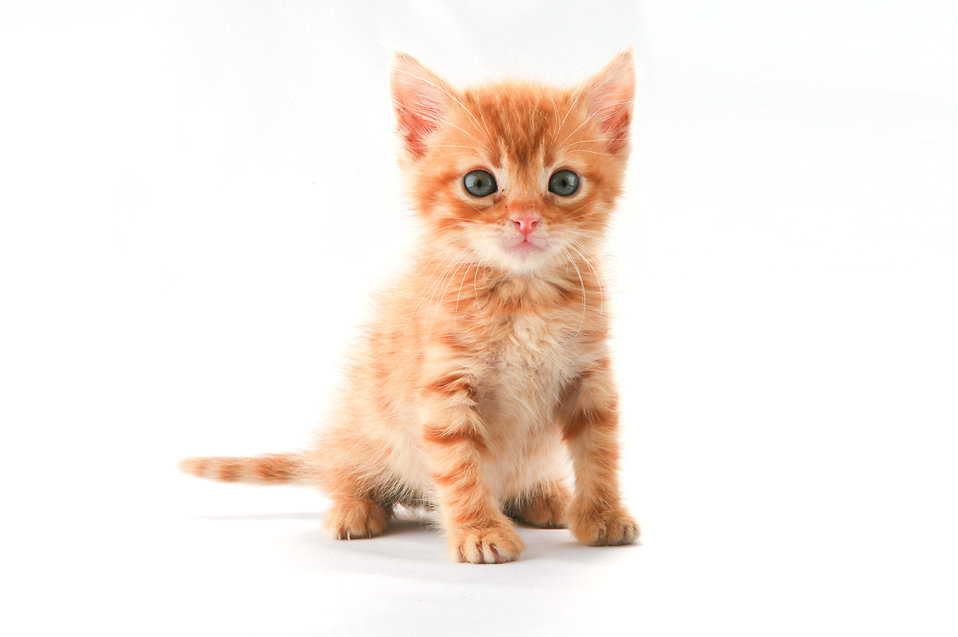
\includegraphics[width=0.5\textwidth]{kitten}
        \caption{It's a kitten. You like kittens.}
    \end{figure}

	\section{Equations}

	Here is the transfer function to the control system shown in figure \ref{ptransfer}:

    \begin{equation}
        \label{ptransfer}
        T(s)=\frac{Y(s)}{R(s)}=I(s) \cdot \frac{K_p \cdot P(s)}{1 + K_p \cdot P(s) \cdot H(s)}
    \end{equation}

	As usual, we can use it's number. That was formula \eqref{ptransfer}
	
    \printglossaries
    
    \phantomsection
    \printbibliography[heading=bibintoc]
	

\end{document}


